\documentclass[a4paper]{article}
\usepackage{fontspec}      %% подготавливает загрузку шрифтов Open Type, True Type и др.
\defaultfontfeatures{Ligatures={TeX},Renderer=Basic}  %% свойства шрифтов по умолчанию
\setmainfont[Ligatures={TeX,Historic},
	SmallCapsFont={Brill},
	SmallCapsFeatures={Letters=SmallCaps}]{Brill}
\usepackage{alltt}
\usepackage{geometry} % Простой способ задавать поля
	\geometry{top=25mm}
	\geometry{bottom=20mm}
	\geometry{left=25mm}
	\geometry{right=20mm}
	\geometry{headsep=25mm}
\usepackage{setspace} % Интерлиньяж
\onehalfspacing % Интерлиньяж 1.5
%\doublespacing % Интерлиньяж 2
%\singlespacing % Интерлиньяж 1
%\usepackage{natbib}
%\bibpunct[: ]{[}{]}{;}{a}{}{,}
\usepackage{enumitem}
\usepackage{array,tabularx,tabulary,booktabs} % Дополнительная работа с таблицами
\usepackage{longtable}  % Длинные таблицы
\usepackage{multirow} % Слияние строк в таблице
\usepackage{multicol} % Несколько колонок
\usepackage{hyperref}
 \usepackage{graphicx}
\setlist{nosep}
\usepackage{titlesec}
\titlespacing*{\section}
{0pt}{2ex plus 0ex minus .2ex}{0ex plus .2ex}
\titlespacing*{\subsection}
{0pt}{2ex plus 0ex minus .2ex}{0ex plus .2ex}
\titlespacing*{\subsubsection}
{0pt}{2ex plus 0ex minus .2ex}{0ex plus .2ex}
\usepackage{sectsty}
\sectionfont{\centering}
\renewcommand{\thesection}{\Roman{section}.}
\renewcommand \thesubsection{\arabic{section}.\arabic{subsection}}

\begin{document}
\begin{center}
{\Large Программа дисциплины <<R, визуализация и статистика>>}
\end{center}
\begin{flushright}
\begin{tabular}{l}
Утверждена                          \\
Академическим советом ОП            \\
Протокол № 15 от  «28» июня 2018 г.
\end{tabular}
\end{flushright}
\begin{center}
\begin{tabular}{|l|l|}
\hline
Автор                         & Г. А. Мороз                    \\ \hline
Число кредитов                &                               \\ \hline
Контактная работа (час.)      &                   40           \\ \hline
Самостоятельная работа (час.) &                 28             \\ \hline
Курс                          & дополнительное образование \\ \hline
Формат изучения дисциплины    & без использования онлайн-курса \\ \hline
\end{tabular}
\end{center}
\section{ЦЕЛЬ И РЕЗУЛЬТАТЫ ОСВОЕНИЯ ДИСЦИПЛИНЫ}
Задачей курса <<R, визуализация и статистика>> является познакомить слушателей с основами R, методами преобразования, визуализации и анализа данных.
\section{СОДЕРЖАНИЕ УЧЕБНОЙ ДИСЦИПЛИНЫ}
\begin{enumerate}
\item Введение в R и RStudio. Вектор. Датафрем. Установка и работа с пакетами
\item Пользовательские функции. Пакет tidyverse
\item Визуализация. Пакет ggplot2, rmarkdown. plotly. shiny
\item Работа со строками. Пакет stringr и stringi
\item Расстояния, регулярные выражения
\item Работа с текстами
\item Описантельная статистика. Фриквентистская статистика
\item Корреляция и регрессия
\end{enumerate}
\section{ОЦЕНИВАНИЕ}
Результирующая оценка выставляется на основании экзамена. Способ округления всех оценок: арифметический.
\section{ПРИМЕРЫ ОЦЕНОЧНЫХ СРЕДСТВ}
\begin{itemize}
\item Постройте следующий график на основании \href{https://tinyurl.com/y8oqsczd}{следующего датасета}:\\
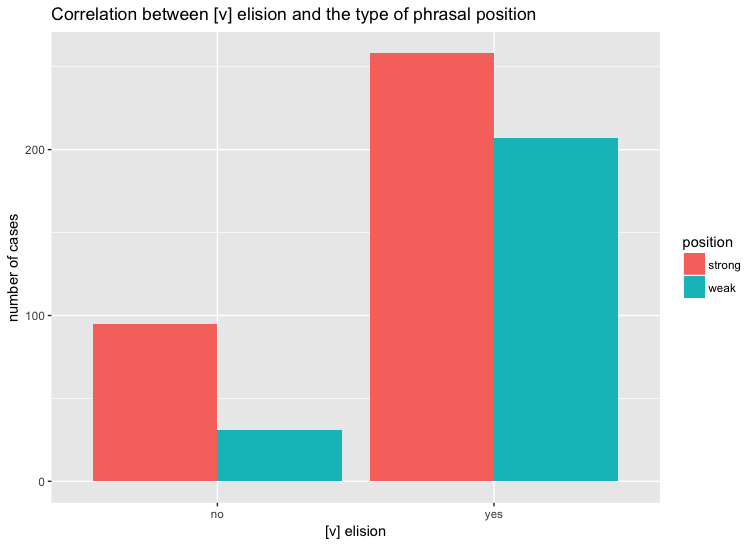
\includegraphics[width=0.5\linewidth]{volition.png}
\item Посчитайте значение корреляции двух переменных встроенного датасета \texttt{ggplot2::diamonds}: depth и price.
\end{itemize}
\section{РЕСУРСЫ}
\subsection{Основная литература}
\begin{itemize}
\item   Bivand, R. S. Applied spatial data analysis with R / R. S. Bivand, E. J. Pebesma, V. Gomez-Rubio. – New York: Springer, 2008. – 374 с. – (Use R!) . – На англ. яз. - ISBN 978-0-387-78170-9. 
\item   Wickham, H.  R for data science: import, tidy, transform, visualize, and model data / H. Wickham, G. Grolemund. – Sebastopol: O'Reilly, 2017. – 492 с. – На англ. яз. - ISBN 9781491910399: 2002.55. 
\end{itemize} 
\subsection{Дополнительная литература}
\begin{itemize}
\item   Xie, Y. Dynamic documents with R and knitr / Y. Xie. – Boca Raton; London; New York: CRC Press, 2014. – 190 с. – (The R series) . – На англ. яз. - ISBN 978-1-482-20353-0. 
\item Spector, P.  Data manipulation with R / P. Spector. – New York: Springer, 2008. – 152 с. – (Use R!) . – На англ. яз. - ISBN 978-0-387-74730-9. 
\item   Wickham, H. ggplot2: elegant graphics for data analysis / H. Wickham. – Dordrecht: Springer, 2009. – 212 с. – (Use R!) . – На англ. яз. - ISBN 978-0-387-98140-6. 
\item   Wickham, H. Advanced R / H. Wickham. – Boca Raton [etc.]: CRC Press, 2014. – 456 с. – (Chapman \& Hall/CRC. The R Series) . – На англ. яз. - ISBN 978-1-466-58696-3. 
\end{itemize}
\subsection{Программное обеспечение}
\begin{tabular}{|l|l|l|}
\hline
№ п/п &	Наименование	& Условия доступа \\ \hline
1	& R &	Свободно распространяемое ПО \\ \hline
2	& Rstudio &	Свободно распространяемое ПО \\ \hline
\end{tabular}
\subsection{Профессиональные базы данных, информационные справочные системы, интернет-ресурсы (электронные образовательные ресурсы)}

\begin{tabular}{|l|l|l|}
\hline
№ п/п &	Наименование	& Условия доступа \\ \hline
1	& Страница курса &	https://agricolamz.github.io/2019\_FE\_R\_statistics/ \\ \hline
\end{tabular}

\subsection{Материально-техническое обеспечение дисциплины}
Учебные аудитории для лекционных занятий по дисциплине обеспечивают использование и демонстрацию тематических иллюстраций, соответствующих программе дисциплины в составе:
\begin{itemize}
\item ПЭВМ с доступом в Интернет (операционная система, офисные программы, антивирусные программы);
\item мультимедийный проектор с дистанционным управлением.
\end{itemize}
Учебные аудитории для лабораторных и самостоятельных занятий по дисциплине оснащены ­­­­­­­­­­­­­­­­­­­­­­­­ ПЭВМ, с возможностью подключения к сети Интернет и доступом к электронной информационно-образовательной среде НИУ ВШЭ.  
\end{document}
